\begin{abstract}
Long-term memory lets LLM agents recall what users told them in earlier sessions. Memory benchmarks, however, are entirely in English, while hundreds of millions of users write code-mixed text such as Hinglish, usually in Latin script. We introduce \lipi{}, a controlled benchmark for cross-lingual and cross-script recall in agent memory. Each of its 240 personal facts about 40 synthetic users is written in nine parallel forms: English, plus a $2\times2$ grid of code-mixed versus monolingual and Latin versus native script for Hindi and for Kannada. The facts are planted in per-user memory pools that stay identical across forms. Across nine retrievers, facts stated in Hindi or Kannada are far harder to retrieve with an English question than the same facts stated in English: mean Recall@5 of multilingual encoders falls from \EnAvgRaw\% to \MitAvgRaw\%. BM25 finds almost nothing, and the English-only default encoder of a popular memory framework cannot retrieve native-script facts at all. A controlled decomposition shows that romanization, not code-mixing, drives the loss. Code-mixed memories are \emph{easier} to retrieve than monolingual ones, Latin script is harder than native script, and Romanized monolingual text is nearly unretrievable. Because an LLM reader answers \EtoEOracleNonEn\% of questions once the right memory is in its context, retrieval is the bottleneck. Deterministic script unification makes retrieval worse, whereas indexing a short LLM-written English gloss next to each non-English memory raises Recall@5 to \MitAvgGloss\%, on par with English-stated facts, and end-to-end accuracy from \EtoERawNonEn\% to \EtoEGlossNonEn\%. We release the benchmark, code and every LLM output.
\end{abstract}

\section{Introduction}
\label{sec:intro}

Long-term memory is what lets an LLM agent behave like the same assistant from one week to the next. Memory-equipped agents write what users tell them into an external store and, when a later request needs it, retrieve the relevant entries back into the context window \citep{park2023generative,packer2023memgpt,chhikara2025mem0,xu2025amem,rasmussen2025zep}. Benchmarks for this capability have multiplied. LoCoMo \citep{maharana2024locomo}, LongMemEval \citep{wu2025longmemeval} and MemoryAgentBench \citep{hu2026memoryagentbench} test recall, temporal reasoning, knowledge updates and selective forgetting. A recent wave of work also studies memories that silently become false \citep{chao2026stale,yadav2026memstrata,sun2026stateauditor,liu2026pacmi}. Every one of these benchmarks is in English.

Many people do not talk to assistants in English. Across India, a dominant written chat register is \emph{code-mixed} Hindi--English (``Hinglish'') or Kannada--English. It is usually typed in Latin script (``Romanized''), sometimes in native script with English words embedded \citep{bali2014borrowing}. Consider a user who writes, in one session, ``\emph{Finally last week Pune shift ho gayi, office se das minute pe flat mil gaya}'', and weeks later asks, in English, ``\emph{Which city do I live in now?}''. The fact is in memory. Whether the agent finds it depends on whether its retriever can relate a Romanized Hindi sentence to an English question, and this has not been measured.

There are reasons to expect trouble. LLMs degrade on Romanized code-mixed instructions, increasingly so as mixing grows \citep{das2026indiromcom}, and a study of sixteen open models attributes most of the loss to romanization rather than to mixing itself \citep{codemixtax2026}. In the evaluation of a production memory engine, a widely used multilingual encoder retrieved only 5\% of Telugu queries correctly \citep{kim2026tablet2}. Deployed memory systems also make design choices that interact with these weaknesses. Mem0 instructs its fact extractor to ``record the facts in the same language'' as the user, and in its input-language mode to preserve ``both the mixed language style AND the script'' of Hinglish input \citep{mem0repo}. A-Mem indexes memories with an English-only sentence encoder by default \citep{amemrepo}.

We introduce \lipi{}, named after the word for ``script'' in both Hindi (\devlipi) and Kannada (\kanlipi). It is a controlled benchmark for cross-lingual and cross-script recall in agent memory, and its central design choice is \emph{parallelism}. Each of 240 personal facts about 40 synthetic users is written in nine forms with identical content: English, and for each of Hindi and Kannada a $2\times2$ grid crossing code-mixing (code-mixed or monolingual) with script (Latin or native). The facts are planted in per-user memory pools of 336 utterances, made of conversational distractors and other users' facts. The pools stay identical across conditions, so any change in retrieval can be attributed to the language and script of the stored memory alone. Questions come in English, the main setting, and also in code-mixed and native-script forms.

Using \lipi{}, we evaluate nine retrievers: BM25, an English-only encoder, five multilingual encoders and two Indic-specialised encoders. We also test three mitigations a memory system could deploy: deterministic script unification, an LLM-written English gloss stored next to each non-English memory, and read-time query translation. Finally, an LLM reader shows how retrieval failures turn into wrong answers.

Our findings are:
\begin{enumerate}
\item \textbf{Facts stated outside English are much harder to find.} Mean Recall@5 of multilingual encoders falls from \EnAvgRaw\% for English-stated facts to \MitAvgRaw\% for the same facts in Hindi or Kannada. The English-only encoder used by default in A-Mem cannot retrieve native-script facts at all.
\item \textbf{Romanization, not code-mixing, drives the loss.} Code-mixed memories are retrieved \emph{more} often than monolingual ones, because embedded English words anchor them, and native script beats Latin script. Romanized monolingual text, which has neither aid, is nearly unretrievable. A tokeniser analysis shows that Romanized Indic words are split into more and less meaningful pieces.
\item \textbf{The fix belongs at write time.} Deterministic script unification makes retrieval worse. A short English gloss written by an LLM when the memory is stored raises Recall@5 to \MitAvgGloss\%, on par with English-stated facts. The benefit holds as memories grow to more than \PoolNLarge{} per user.
\item \textbf{Retrieval, not reading, is the bottleneck.} An LLM reader answers \EtoEOracleNonEn\% of questions correctly once the right memory is in context, and end-to-end accuracy on non-English facts rises from \EtoERawNonEn\% to \EtoEGlossNonEn\% with the gloss.
\end{enumerate}

Our contributions are \lipi{}, the first benchmark for long-term memory over code-mixed and Romanized conversations, and a controlled study that separates the effects of code-mixing, script and language on memory retrieval with paired statistics. We also evaluate inexpensive mitigations and identify one that closes the gap at a cost of one short LLM call per non-English memory. We release all data, prompts, LLM outputs and code, so that every number in the paper can be regenerated without API access.

\section{Related Work}
\label{sec:related}

\paragraph{Long-term memory for LLM agents.}
Memory architectures range from reflection-based memory streams \citep{park2023generative} and operating-system-style paging \citep{packer2023memgpt} to extraction-and-update pipelines \citep{chhikara2025mem0}, self-organising note graphs \citep{xu2025amem} and temporal knowledge graphs \citep{rasmussen2025zep}; \citet{zhang2024memorysurvey} survey the area. Almost all of them retrieve memories by dense similarity with an off-the-shelf sentence encoder.

Evaluation has focused on English conversations. LoCoMo tests very long dialogues \citep{maharana2024locomo}, LongMemEval tests five memory abilities over chat histories of up to 1.5M tokens \citep{wu2025longmemeval}, and MemoryAgentBench adds test-time learning and conflict resolution \citep{hu2026memoryagentbench}. A 2026 line of work targets memories that become invalid: STALE isolates implicit invalidation \citep{chao2026stale}, MemStrata retires superseded facts deterministically \citep{yadav2026memstrata}, and MemTX, StateAuditor and PACMI propose transactional, post-hoc and provenance-based repair \citep{li2026memtx,sun2026stateauditor,liu2026pacmi}.

The closest multilingual evaluation, Wontopos Tablet-2 \citep{kim2026tablet2}, measures a production memory engine across 14 languages using native-speaker captions, but does not consider code-mixed or Romanized text. To our knowledge, \lipi{} is the first memory benchmark in which the language and script of the \emph{stored} memory differ from those of the question.

\paragraph{Code-mixing and romanization.}
Code-mixing is pervasive in Indian social media \citep{bali2014borrowing}, and benchmarks such as GLUECoS and LinCE cover classification and tagging tasks on it \citep{khanuja2020gluecos,aguilar2020lince}. Recent LLM-era studies find consistent degradation on Romanized code-mixed instructions \citep{das2026indiromcom} and attribute it mainly to romanization \citep{codemixtax2026}. Conversely, RomanSetu shows that romanized inputs can be an efficient bridge for extending LLMs to Indic languages \citep{husain2024romansetu}.

Tooling is asymmetric. Transliteration models convert between native and Latin script \citep{madhani2023aksharantar}, and strong Indic machine translation systems such as IndicTrans2 expect native-script input \citep{gala2023indictrans2}, but code-mixed text has no standard canonical form. In information retrieval, mixed-script queries were studied in the FIRE shared tasks and for web search \citep{gupta2014mixedscript}, before the advent of dense retrieval and agent memory.

\paragraph{Multilingual dense retrieval.}
Several encoder families are trained for cross-lingual alignment. LaBSE uses translation pairs \citep{feng2022labse}, and multilingual SBERT models are distilled from English ones \citep{reimers2020multilingual}. mE5 \citep{wang2024me5}, BGE-M3 \citep{chen2024bgem3} and Qwen3-Embedding \citep{zhang2025qwen3embedding} are trained at scale and evaluated on MIRACL \citep{zhang2023miracl} and MTEB-style suites. Indic-specialised encoders include L3Cube-IndicSBERT \citep{deode2023indicsbert} and Vyakyarth \citep{krutrim2025vyakyarth}. Their training data is overwhelmingly native-script, and how they behave on Romanized or code-mixed \emph{memories} queried in English is exactly what \lipi{} measures.

\section{The \lipi{} Benchmark}
\label{sec:benchmark}

\subsection{Design goals}
We want to measure one thing cleanly: whether a memory system can retrieve a fact when the language or script in which the user stated it differs from the language of the later question. Four requirements follow.
\begin{itemize}
\item \textbf{Parallel forms.} Every condition contains the same facts, so differences cannot come from content.
\item \textbf{Fixed pools.} Every condition uses the same distractors, so only the target memory changes.
\item \textbf{Realistic distractors.} Distractors include code-mixed chat in both scripts, and other users' personal facts serve as hard negatives.
\item \textbf{Unambiguous answers.} Answers are short and come with alias lists, so end-to-end accuracy can be scored without an LLM judge.
\end{itemize}

\subsection{Users, facts and the nine forms}
\lipi{} has 40 synthetic users (20 female, 20 male), each with six personal facts from 24 relation types: home city, hometown, employer, job, a pet's name, a sibling's name, a partner's name, allergy, diet, favourite dish, an instrument being learned, weekend sport, a recently bought vehicle, the next trip, an exam being prepared for, an injury, workout time, favourite singer, a language being learned, a child's name, commute mode, favourite team, college and savings goal. A balanced design assigns every relation type to exactly 10 users, giving 240 facts.

Each fact is a short first-person chat message to an assistant that states the fact with a little everyday context (median 21 words in English). It is written in nine parallel forms (Table~\ref{tab:example}): English (\form{EN}), and for each language $L\in\{$Hindi (\form{hi}), Kannada (\form{kn})$\}$ four forms crossing code-mixing with script:
\begin{itemize}
\item \form{$L$-CM-R}: code-mixed text in Latin script.
\item \form{$L$-CM-N}: the same words, with $L$ words and names in native script and English words left in Latin script.
\item \form{$L$-MO-N}: monolingual $L$ in native script.
\item \form{$L$-MO-R}: the same words as \form{$L$-MO-N}, romanized casually.
\end{itemize}

The code-mixed forms use colloquial chat vocabulary; 35\% (Hindi) and 40\% (Kannada) of their Latin-script tokens are common English words. The monolingual forms replace English words with native vocabulary wherever a common word exists, leaving 15\% and 8\% English tokens, mostly unavoidable loanwords and brand names. Hindi first-person verbs agree with the user's gender.

Each fact also has an English question (e.g.\ ``\emph{Which city do I live in now?}'') and, for each language, a code-mixed Latin-script question and a monolingual native-script question. Questions never contain the answer and, following LongMemEval \citep{wu2025longmemeval}, are written to share few content words with the statement. Answers are short, such as a name, a city or a time, and come with alias lists that cover spelling variants and native-script spellings.

\begin{table}[t]
\centering
\small
\caption{One \lipi{} fact (user u02, relation \emph{home city}, answer \emph{Pune}) in its nine parallel forms, with its questions. \form{CM-R} and \form{CM-N} (likewise \form{MO-N} and \form{MO-R}) use the same words in different scripts.}
\label{tab:example}
\begin{tabular}{@{}l l >{\raggedright\arraybackslash}p{10.6cm}@{}}
\toprule
Form & Type & Memory text \\
\midrule
\form{EN} & English & Finally shifted to Pune last week, found a flat just ten minutes from the office. \\
\midrule
\form{hi-CM-R} & code-mixed, Latin & Finally last week Pune shift ho gayi, office se das minute pe flat mil gaya. \\
\form{hi-CM-N} & code-mixed, native & \adjustbox{valign=t}{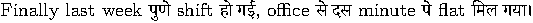
\includegraphics{indic/ex_hi_cm_nat.pdf}} \\
\form{hi-MO-N} & monolingual, native & \adjustbox{valign=t}{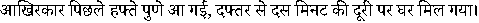
\includegraphics{indic/ex_hi_mono_nat.pdf}} \\
\form{hi-MO-R} & monolingual, Latin & aakhirkaar pichhle hafte Pune aa gayi, daftar se das minute ki doori par ghar mil gaya. \\
\midrule
\form{kn-CM-R} & code-mixed, Latin & Finally last week Pune ge shift aade, office inda hattu nimisha dooradalli flat sikkitu. \\
\form{kn-CM-N} & code-mixed, native & \adjustbox{valign=t}{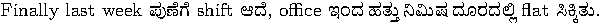
\includegraphics{indic/ex_kn_cm_nat.pdf}} \\
\form{kn-MO-N} & monolingual, native & \adjustbox{valign=t}{
\includegraphics{indic/ex_kn_mono_nat.pdf}} \\
\form{kn-MO-R} & monolingual, Latin & konegu kaleda vaara Punege bande, kacheriyinda hattu nimishada dooradalli mane sikkitu. \\
\midrule
Question & EN & Which city do I live in now? \\
Question & hi-CM-R / hi-MO-N & \adjustbox{valign=t}{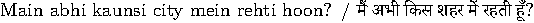
\includegraphics{indic/ex_q_hi.pdf}} \\
Question & kn-CM-R / kn-MO-N & \adjustbox{valign=t}{
\includegraphics{indic/ex_q_kn.pdf}} \\
\bottomrule
\end{tabular}
\end{table}


\subsection{Memory pools}
\label{sec:pools}
For each user and each language $L$ we build a memory pool of 336 utterances. The memory unit is a single user message, as in turn-level indexing \citep{wu2025longmemeval}. A pool contains three groups:
\begin{itemize}
\item the user's \textbf{six facts}, all in the condition's form;
\item \textbf{30 hard negatives}: personal facts of other users with relation types the user does not have, spread evenly over the five forms of $L$;
\item \textbf{300 distractors}: 100 English utterances from Synthetic-Persona-Chat \citep{jandaghi2023syntheticpersonachat}, and 100 Romanized and 100 native-script turns from the friends and family conversations of IndicTalk \citep{gawande2026indictalk} in language $L$.
\end{itemize}

Long distractor turns are split into one- or two-sentence chunks of 8--35 words so that their length matches the facts, and emoji are removed. To keep every question answerable from a single memory, we drop from each user's pool any distractor that contains one of the user's answer aliases or touches one of the user's relation topics, using keyword filters in three languages and both scripts.

The pools are \emph{identical across the five forms of a language}: switching a condition from \form{EN} to \form{hi-CM-R} replaces only the user's six facts. Comparisons between forms are therefore paired at the level of individual facts.

\subsection{Construction and quality control}
\label{sec:quality}
The 240 facts were drafted by Claude models following a written style guide (Appendix~\ref{app:style}): 39 by Claude Opus and 201 by Claude Sonnet. Every fact passes automatic checks:
\begin{itemize}
\item all 19 fields are present;
\item Latin-script forms contain no Indic characters;
\item native-script monolingual forms are at least 85\% native characters;
\item code-mixed native forms mix the two scripts;
\item each Romanized code-mixed form has a higher English-token ratio than its monolingual counterpart;
\item the paired forms (\form{CM-R}/\form{CM-N}, \form{MO-N}/\form{MO-R}) have matching word counts after transliteration;
\item an answer alias occurs in all nine forms;
\item no question contains its answer;
\item no first-person verb disagrees with the user's gender.
\end{itemize}

An independent LLM review (Claude Sonnet, prompted as a Hindi or Kannada linguist) of 30 facts per language flagged 2 of the 180 Hindi strings (1.1\%) and 8 of the 180 Kannada strings (4.4\%). Most flags were romanization mismatches between paired forms; one was a missing case ending and one an unnatural word choice. All flagged strings were corrected before the experiments reported here. A native-speaker study is left to future work. To support it, we release review sheets with 72 facts per language.

\section{Experimental Setup}
\label{sec:setup}

\paragraph{Retrievers.}
Table~\ref{tab:retrievers} lists the nine retrievers:
\begin{itemize}
\item BM25 \citep{robertson2009bm25} with Unicode-aware tokenisation;
\item \texttt{all-MiniLM-L6-v2} \citep{wang2020minilm,reimers2019sbert}, the English-only default encoder of A-Mem;
\item five multilingual encoders: paraphrase-multilingual-MiniLM \citep{reimers2020multilingual}, mE5-small and mE5-base \citep{wang2024me5}, LaBSE \citep{feng2022labse} and BGE-M3 (dense) \citep{chen2024bgem3};
\item two Indic-specialised encoders: IndicSBERT \citep{deode2023indicsbert} and Vyakyarth \citep{krutrim2025vyakyarth}.
\end{itemize}
Dense retrieval uses cosine similarity with the prefixes each model recommends.

\begin{table}[t]
\centering
\small
\setlength{\tabcolsep}{4pt}
\caption{Retrievers evaluated. Parameter counts are approximate.}
\label{tab:retrievers}
\begin{tabular}{@{}l l l l l@{}}
\toprule
Short name & Model & Type & Params & Notes \\
\midrule
bm25 & \texttt{BM25} & lexical & -- & \citet{robertson2009bm25} \\
MiniLM-en & \texttt{all-MiniLM-L6-v2} & English-only & 23M & A-Mem default \\
mMiniLM & \texttt{paraphrase-multilingual-MiniLM-L12-v2} & multilingual & 118M & 50+ languages \\
mE5-small & \texttt{multilingual-e5-small} & multilingual & 118M & \texttt{query:}/\texttt{passage:} prefixes \\
mE5-base & \texttt{multilingual-e5-base} & multilingual & 278M & \texttt{query:}/\texttt{passage:} prefixes \\
LaBSE & \texttt{LaBSE} & multilingual & 471M & translation-pair trained \\
BGE-M3 & \texttt{bge-m3 (dense)} & multilingual & 568M & XLM-R large backbone \\
IndicSBERT & \texttt{indic-sentence-similarity-sbert} & Indic & 238M & L3Cube; 10 Indic languages \\
Vyakyarth & \texttt{Vyakyarth} & Indic & 278M & Krutrim; XLM-R based \\
\bottomrule
\end{tabular}
\end{table}


\paragraph{Task and metrics.}
For each fact, stored form and question form, we rank the user's whole memory pool against the question and record the rank of the target utterance. We report Recall@$k$, the probability that the target is among the top $k$, for $k\in\{1,5,10\}$, together with mean reciprocal rank (MRR). Recall@5 is our headline metric because memory systems typically pass a handful of memories to the reader. Uncertainty is quantified with 95\% bootstrap confidence intervals over the 240 facts (2{,}000 resamples), and paired comparisons between forms use McNemar's exact test on per-fact Recall@5 outcomes.

\paragraph{Mitigations.}
All mitigations change only how memories and questions are indexed; the stored text shown to the reader is never replaced. We compare five variants:
\begin{itemize}
\item \textbf{Raw}: memories and questions are embedded as written.
\item \textbf{Translit}: script unification. Every native-script span in memories and questions is deterministically romanized, using ITRANS transliteration followed by casual-spelling rules, diacritic removal and Hindi word-final schwa deletion.
\item \textbf{Gloss}: write-time canonicalisation. When a memory is written, an LLM produces a faithful English gloss; both the raw memory and the gloss are indexed, and a memory's score is the maximum of the two similarities. A cheap English-word-ratio language-identification check skips memories that already look English; it routed 4{,}294 of the 5{,}160 memory utterances to the LLM.
\item \textbf{QT}: read-time translation of non-English questions into English, with the score taken as the maximum over the original and the translated question.
\item \textbf{Gloss+QT}: the two combined.
\end{itemize}

Glosses and question translations were produced by Claude Haiku 4.5 (\texttt{claude-haiku-4-5-20251001}). The model saw only the memory text, under opaque identifiers, so it could not tell facts from distractors and saw no questions or answers. Generation ran through a sub-agent interface with default sampling. Automatic checks rejected 969 first-pass outputs that were placeholders rather than translations, and these were regenerated. In the final glosses, a Latin-script answer alias survives in \glossKeep{} of the 1{,}919 glossed non-English facts (Appendix~\ref{app:gloss}). All 5{,}254 outputs are released, so downstream numbers are exactly reproducible.

\paragraph{End-to-end reading.}
To see how retrieval errors become answer errors, we sample 48 facts (two per relation type). An LLM reader (Claude Haiku 4.5) receives the English question together with five memories under three conditions:
\begin{itemize}
\item \textbf{Raw}: the top 5 retrieved by mE5-base with Raw indexing;
\item \textbf{Gloss}: the top 5 retrieved with Gloss indexing;
\item \textbf{Oracle}: the target memory plus four random memories from the same pool.
\end{itemize}
The reader always sees the raw memory texts, so the conditions differ only in what was retrieved. Answers are scored by alias match.
